%%%%%%%%%%%%%%%%%%%%%%%%%%%%%%%%%%%%%%%%%%%%%%%%%%%%%%%%%%%%%%%%%%%%%%%%%%%%%%%%%%%%%%%%%%%%%
%%									Chapitre 2											%
%%%%%%%%%%%%%%%%%%%%%%%%%%%%%%%%%%%%%%%%%%%%%%%%%%%%%%%%%%%%%%%%%%%%%%%%%%%%%%%%%%%%%%%%%%%%%
\chapter{Stochastic Multi-Armed Bandits}\label{chap:mab}
	\citationChap{
	blabla
	}{}
	\minitoc
	\newpage

%%%%%%%%%%%%%%%%%%%%%%%%%%%%%%%%%%%%%%%%%%%%%%%%%%%%%%%%%%%%%%%%%%%%%%%%%%%%%%%%%%%%%%%%%%%%%

\section{The Multi-Armed Bandits Model}\label{sec:mab.model}

The problem of sequentially allocating resources to a defined set of actions (arms) based on successive \emph{partially observable} (see Definition~\ref{def:mab.mab} and Remark~\ref{remark:mab.partial} below) feedback refers to the MAB problem in probability theory. The term \emph{bandit} is named, by analogy, after slot machines (or one-armed bandits) in a casino. A sequential decision making problem comes up then when facing with several slot machines (multi-armed bandits).

The study of MAB models can date back to 1933~\citep{thompson1933}, and was first proposed to deal with clinical trials. 

\begin{figure}
    \centering
    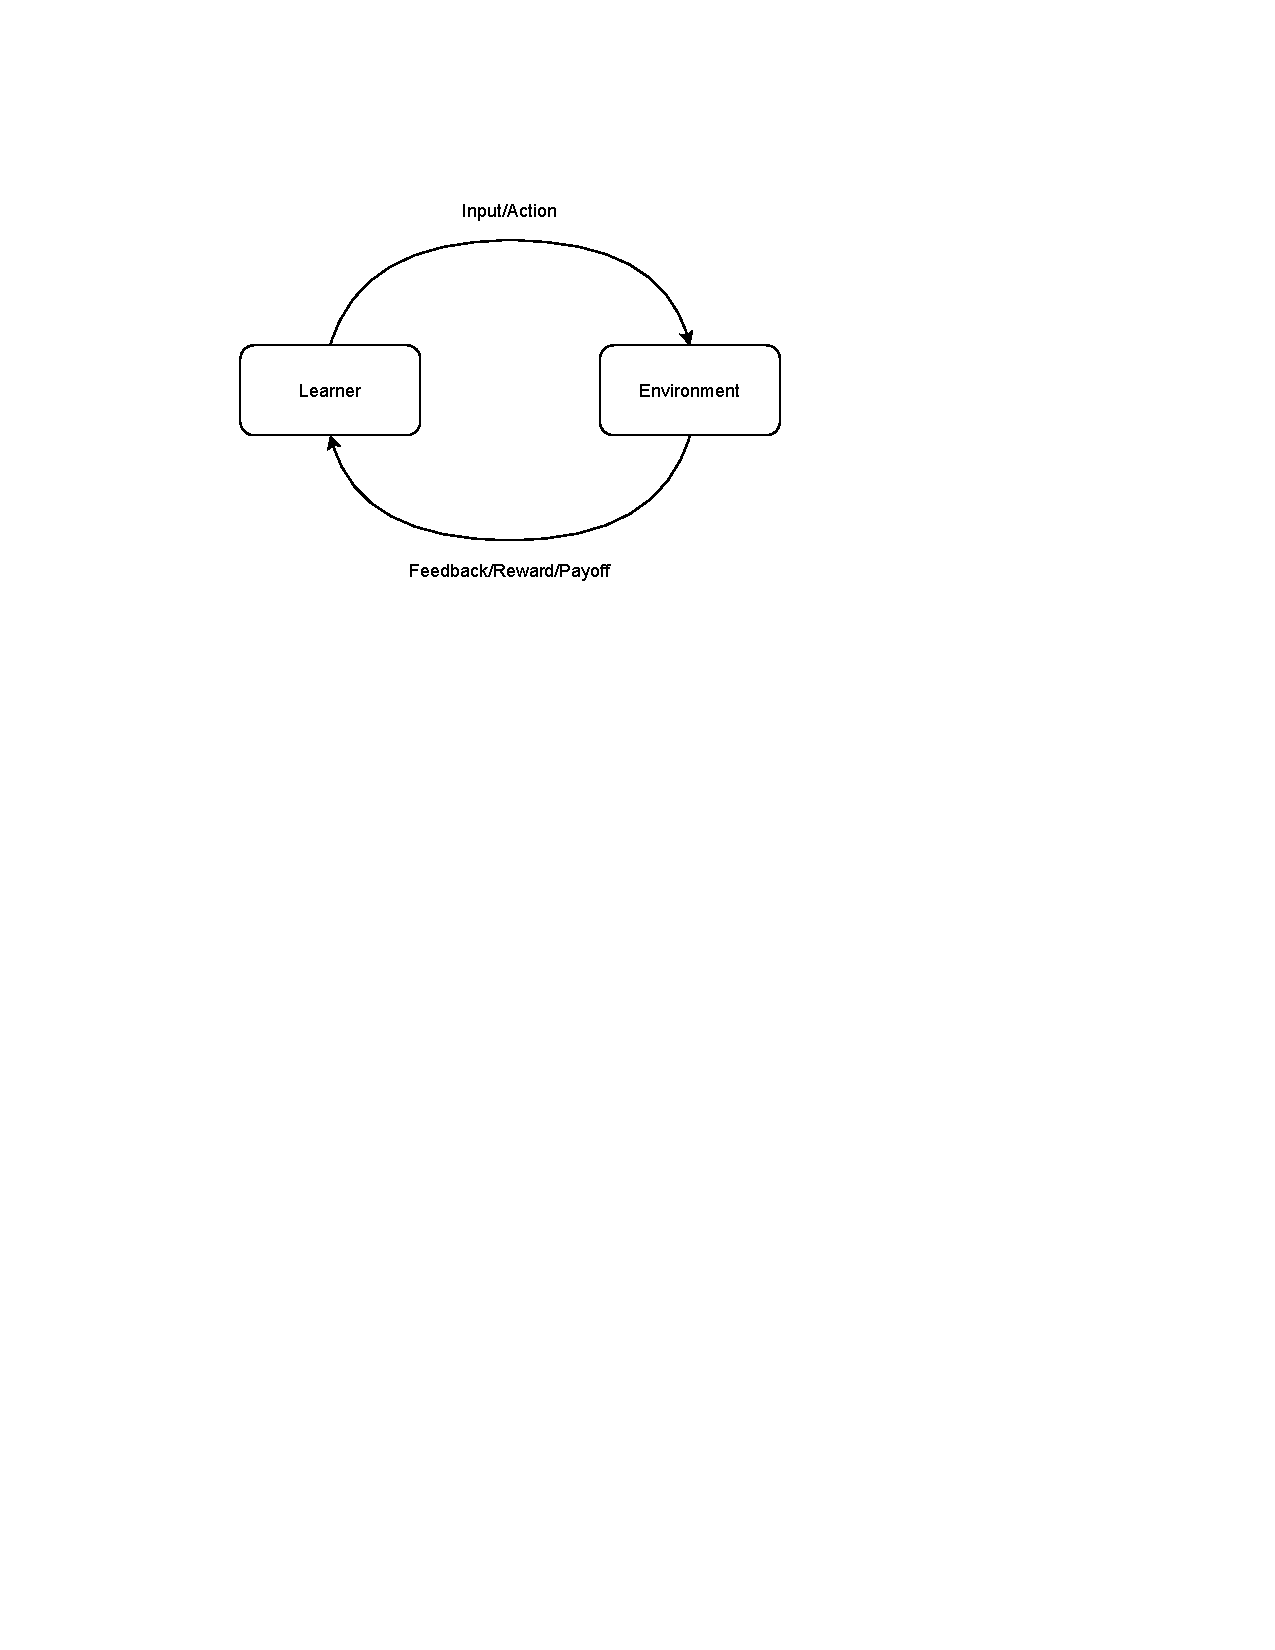
\includegraphics[width=0.5\textwidth]{Chapter2/img/mab.pdf}
    \caption{A bandit learning cycle.}
    \label{fig:mab.mab}
\end{figure}

As stated in Chapter~\ref{chap:intro}, the original learning goal in stochastic MAB is to maximize the total payoff obtained given a sequence of observations. For that purpose, the learner is required to balance between exploration and exploitation.

In this section, we go beyond the intuition and provide the formal definition of the model. We also recall some fundamental results for the sake of self-containedness.

\subsection{Problem Formulation}\label{sec:mab.model.formulation}

An MAB problem can be formulated as follow.

\begin{definition}[multi-armed bandit problem]\label{def:mab.mab}
\begin{leftbar}[defnbar]
	We are given a set of $K$ arms $\{1,\ldots,K\}$ that follow $K$ unknown $[0,1]$-valued distributions $(\nu_k)_{1 \leq k \leq K}$, and a time horizon $T$. At each time step $t$, the process consists of the following actions:
	\begin{itemize}
		\item a vector of rewards $(r_{1,t} \sim \nu_1, \ldots, r_{K,t} \sim \nu_K)$ is generated,
		\item the learner picks an arm $k_t \in \{1,\ldots,K\}$, and
		\item the learner observes the reward $r_t = r_{k_t, t}$.
	\end{itemize}
\end{leftbar}
\end{definition}

\begin{remark}\label{remark:mab.partial}
\begin{leftbar}[remarkbar]
	Rewards of unchosen arms at time $t$ are not revealed, this partial feedback setting is a special case of the online learning with experts setting.
\end{leftbar}
\end{remark}

\subsection{Regret minimization}\label{sec:mab.model.regret}

As we have mentioned in Chapter~\ref{chap:intro} that one needs to trade-off between exploration and exploitation in a MAB problem. The objective is to design a clever (in a precise sense) way of choosing the arms based on the past observations, and we call this design an \emph{allocation strategy} or \emph{policy}. Depending on our ultimate goal, we usually have two criteria of performance measurement for a given policy.

Suppose that each unknown distribution $\nu_k$ is associated with a mean $\mu_k$, and that $\mu^{\star}$ is the mean of the optimal arm. One natural way to assess the quality of the given policy would be minimizing the total loss w.r.t the optimal arm during the whole process, which leads to the notion of \gls{cumulative regret} (sometimes simply called regret if there is no ambiguity).

\begin{definition}[cumulative regret]\label{def:mab.cumulative_regret}
\begin{leftbar}[defnbar]
	At the end of round $T$, a given policy which observes a sequence of rewards $(r_t)_{1 \leq t \leq T}$ suffers from a cumulative regret:
	\[
		\hat{R}_T \eqdef \max_{i=1\cdots K} \sum_{t=1}^T r_{i,t} - \sum_{t=1}^T r_t.
	\]
\end{leftbar}
\end{definition}

In general, both rewards and choices of the learner might be stochastic, it is thus often more convenient to consider a related \emph{pseudo-regret} that involves only the mean rewards $\mu_k$.

\begin{definition}[cumulative pseudo-regret]\label{def:mab.pseudo_regret}
\begin{leftbar}[defnbar]
	At the end of round $T$, a given policy which observes a sequence of rewards $(r_t)_{1 \leq t \leq T}$ suffers from a cumulative pseudo-regret:
	\[
		R_T \eqdef \mu^{\star}T - \sum_{t=1}^T \mu_{k_t}.
	\]
\end{leftbar}
\end{definition}

\begin{proposition}\label{prop:mab.pseudo_regret}
\begin{leftbar}[propositionbar]
	The expected value $\E[\hat{R}_T]$ of the cumulative regret and the expected value $\E[R_T]$ of the cumulative pseudo-regret are the same, where the expectation is taken with respect to both rewards and choices from the learner.
\end{leftbar}
\end{proposition}

\begin{proof}
	Let us define a function that relates each arm to its mean reward \func{f}{\{1,\ldots,K\}}{\R}{k_t}{\mu_{k_t}\,,} then by the tower rule, we have
    \[
	    \E[r_t] = \E[\E[r_t|k_t]] = \E[f(k_t)] = \mu_{k_t}\,.
    \]
\end{proof}

In practice, people are essentially interested in bounding: (a) the \emph{expected cumulative regret}, or (b) the \emph{cumulative regret with high probability}. One can notice that the two definitions of cumulative regret above are equivalent if their objective is to obtain an expected regret bound. Hence, people often only focus on the pseudo-regret. 


\subsection{\UCB{} and asymptotically optimal strategy}\label{sec:mab.model.ucb}

\section{Multi-Armed Bandits for Optimization}\label{sec:mab.optim}

\subsection{Best-arm identification for stochastic multi-armed bandits}

\subsection{Best-arm identification for linear bandits}

\subsection{Other variants of best-arm identification}

\subsection{$\cX$-armed bandits}

\section{Performance Measure}\label{sec:mab.performance}

\subsection{Optimization error}

\subsection{Sample complexity}

\subsection{Simple regret}

\begin{definition}[simple regret]\label{def:stoch_mab.simple_regret}
\begin{leftbar}[defnbar]
	At the end of round $T$, a given policy which observes a sequence of rewards $(r_t)_{1 \leq t \leq T}$ and a recommendation $j_T$ suffers from a simple regret:
	\[
		S_T \eqdef \mu^{\star} - \mu_{j_T}\,.
	\]
\end{leftbar}
\end{definition}